\chapter{Judges 4}

\begin{figure}
  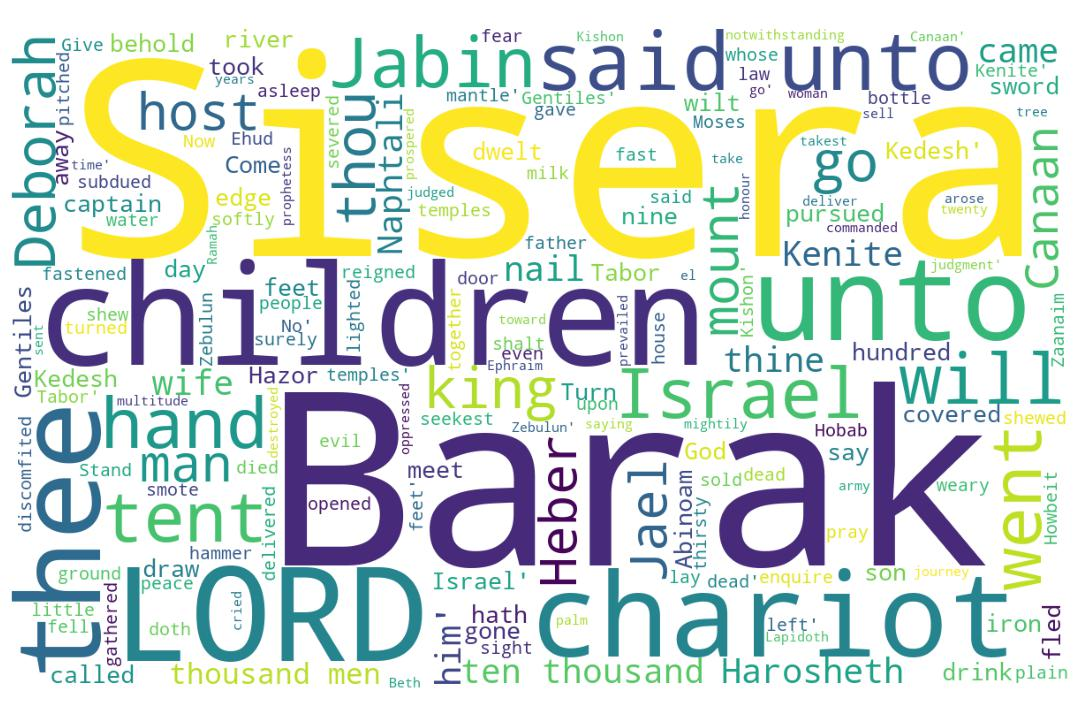
\includegraphics[width=\linewidth]{07OT-Judges/Judges4-WordCloud.jpg}
  \caption{Judges 4 Word Cloud}
  \label{fig:Judges 4 Word Cloud}
\end{figure}


\marginpar{\scriptsize \centering \fcolorbox{bone}{lime}{\textbf{YET AGAIN}}\\ (Judges 4) \begin{compactenum}[I.][8]
    \item   A New  \textbf{Chapter}  \index[scripture]{Judges!Jdg 04:01} (Jdg 4:1) 
    \item   Same  \textbf{Choices}  \index[scripture]{Judges!Jdg 04:01} (Jdg 4:1) 
    \item   The Lord's \textbf{Command}   \index[scripture]{Judges!Jdg 04:06}    (Jdg 4:6) 
    \item   The Enemy  \textbf{Captain}  \index[scripture]{Judges!Jdg 04:06} (Jdg 6:6) 
    \item   The   \textbf{Calls}  \index[scripture]{Judges!Jdg 04:06} \index[scripture]{Judges!Jdg 04:10} (Jdg 4:6, 10) 
    \item   A  \textbf{Champion}  \index[scripture]{Judges!Jdg 04:09} (Jdg 4:9) 
    \item   The  \textbf{Chariots}  \index[scripture]{Judges!Jdg 04:13} (Jdg 4:13) 
\end{compactenum}}


\footnote{\textcolor[rgb]{0.00,0.25,0.00}{\hyperlink{JudgesTOC}{Return to end of Table of Contents.}}}\footnote{\href{https://audiobible.com/bible/judges_4.html}{\textcolor[cmyk]{0.99998,1,0,0}{Judges 4 Audio}}}\textcolor[cmyk]{0.99998,1,0,0}{And the children of Israel \fcolorbox{bone}{lime}{again} did \fcolorbox{bone}{lime}{evil} in the sight of the LORD, when Ehud was dead.}
[2] \textcolor[cmyk]{0.99998,1,0,0}{And the LORD sold them into the hand of Jabin king of Canaan, that reigned in Hazor; the captain of whose host \emph{was} \fcolorbox{bone}{bone}{Sisera}, which dwelt in Harosheth of the Gentiles.}
[3] \textcolor[cmyk]{0.99998,1,0,0}{And the children of Israel cried unto the LORD: for he had nine hundred chariots of iron; and twenty years he mightily oppressed the children of Israel.}\\
\\
\P \textcolor[cmyk]{0.99998,1,0,0}{And Deborah, a prophetess, the wife of Lapidoth, she judged Israel at that time.}
[5] \textcolor[cmyk]{0.99998,1,0,0}{And she dwelt under the palm tree of Deborah between Ramah and Beth-el in mount Ephraim: and the children of Israel came up to her for judgment.}
[6] \textcolor[cmyk]{0.99998,1,0,0}{And she sent and called Barak the son of Abinoam out of Kedesh-naphtali, and said unto him, Hath not the LORD God of Israel \fcolorbox{bone}{lime}{commanded}, \emph{saying}, Go and draw toward mount Tabor, and take with thee ten thousand men of the children of Naphtali and of the children of Zebulun?}
[7] \textcolor[cmyk]{0.99998,1,0,0}{And I will draw unto thee to the river Kishon \fcolorbox{bone}{bone}{Sisera}, the captain of Jabin's army, with his chariots and his multitude; and I will deliver him into thine hand.}
[8] \textcolor[cmyk]{0.99998,1,0,0}{And Barak said unto her, If thou wilt go with me, then I will go: but if thou wilt not go with me, \emph{then} I will not go.}
[9] \textcolor[cmyk]{0.99998,1,0,0}{And she said, I will surely go with thee: notwithstanding the journey that thou takest shall not be for thine honour; for the LORD shall sell \fcolorbox{bone}{bone}{Sisera} into the hand of a woman. And \fcolorbox{bone}{lime}{Deborah} arose, and went with Barak to Kedesh.}\\
\\
\P \textcolor[cmyk]{0.99998,1,0,0}{And Barak \fcolorbox{bone}{lime}{called} Zebulun and Naphtali to Kedesh; and he went up with ten thousand men at his feet: and Deborah went up with him.}
[11] \textcolor[cmyk]{0.99998,1,0,0}{Now Heber the Kenite, \emph{which} \emph{was} of the children of Hobab the father in law of Moses, had severed himself from the Kenites, and pitched his tent unto the plain of Zaanaim, which \emph{is} by Kedesh.}
[12] \textcolor[cmyk]{0.99998,1,0,0}{And they shewed \fcolorbox{bone}{bone}{Sisera} that Barak the son of Abinoam was gone up to mount Tabor.}
[13] \textcolor[cmyk]{0.99998,1,0,0}{And \fcolorbox{bone}{bone}{Sisera} gathered together all his \fcolorbox{bone}{lime}{chariots}, \emph{even} nine hundred chariots of iron, and all the people that \emph{were} with him, from Harosheth of the Gentiles unto the river of Kishon.}\
[14] \textcolor[cmyk]{0.99998,1,0,0}{And Deborah said unto Barak, Up; for this \emph{is} the day in which the LORD hath delivered \fcolorbox{bone}{bone}{Sisera} into thine hand: is not the LORD gone out before thee? So Barak went down from mount Tabor, and ten thousand men after him.}
[15] \textcolor[cmyk]{0.99998,1,0,0}{And the LORD discomfited \fcolorbox{bone}{bone}{Sisera}, and all \emph{his} chariots, and all \emph{his} host, with the edge of the sword before Barak; so that \fcolorbox{bone}{bone}{Sisera} lighted down off \emph{his} chariot, and fled away on his feet.}
[16] \textcolor[cmyk]{0.99998,1,0,0}{But Barak pursued after the chariots, and after the host, unto Harosheth of the Gentiles: and all the host of \fcolorbox{bone}{bone}{Sisera} fell upon the edge of the sword; \emph{and} there was not a man left.}
[17] \textcolor[cmyk]{0.99998,1,0,0}{Howbeit \fcolorbox{bone}{bone}{Sisera} fled away on his feet to the tent of Jael the wife of Heber the Kenite: for \emph{there} \emph{was} peace between Jabin the king of Hazor and the house of Heber the Kenite.}\\
\\
\P \textcolor[cmyk]{0.99998,1,0,0}{And Jael went out to meet \fcolorbox{bone}{bone}{Sisera}, and said unto him, Turn in, my lord, turn in to me; fear not. And when he had turned in unto her into the tent, she covered him with a mantle.}
[19] \textcolor[cmyk]{0.99998,1,0,0}{And he said unto her, Give me, I pray thee, a little water to drink; for I am thirsty. And she opened a bottle of milk, and gave him drink, and covered him.}
[20] \textcolor[cmyk]{0.99998,1,0,0}{Again he said unto her, Stand in the door of the tent, and it shall be, when any man doth come and enquire of thee, and say, Is there any man here? that thou shalt say, No.}
[21] \textcolor[cmyk]{0.99998,1,0,0}{Then Jael Heber's wife took a nail of the tent, and took an hammer in her hand, and went softly unto him, and smote the nail into his temples, and fastened it into the ground: for he was fast asleep and weary. So he died.}
[22] \textcolor[cmyk]{0.99998,1,0,0}{And, behold, as Barak pursued \fcolorbox{bone}{bone}{Sisera}, Jael came out to meet him, and said unto him, Come, and I will shew thee the man whom thou seekest. And when he came into her \emph{tent}, behold, \fcolorbox{bone}{bone}{Sisera} lay dead, and the nail \emph{was} in his temples.}
[23] \textcolor[cmyk]{0.99998,1,0,0}{So God subdued on that day Jabin the king of Canaan before the children of Israel.}
[24] \textcolor[cmyk]{0.99998,1,0,0}{And the hand of the children of Israel prospered, and prevailed against Jabin the king of Canaan, until they had destroyed Jabin king of Canaan.}